\documentclass{beamer}

\usetheme{CambridgeUS}
\usecolortheme{orchid}

%%%%%%%%%%%%%%%%%%%%%%%%%%%%%%%%%%%%%%%%%%%%%%%%%%%%%%%%%%%%%%%%%%%%%%%%%%%%%%%%
% Fonts
%%%%%%%%%%%%%%%%%%%%%%%%%%%%%%%%%%%%%%%%%%%%%%%%%%%%%%%%%%%%%%%%%%%%%%%%%%%%%%%%

\usepackage{polyglossia}
\setmainlanguage{chinese}
\setotherlanguage{hebrew}
\setotherlanguage{greek}
\setotherlanguage{english}

\usepackage{fontspec}
\usefonttheme{professionalfonts}

\newfontfamily\chinesefont{Noto Sans CJK TC}
\newfontfamily\cjkfontsf{Noto Sans CJK TC}
\newfontfamily\cjkfonttt{Noto Sans CJK TC}

\newfontfamily\hebrewfont[Script=Hebrew]{David CLM}
\newfontfamily\hebrewfontsf[Script=Hebrew]{David CLM}

\newfontfamily\greekfont[Script=Greek]{Noto Sans}
\newfontfamily\greekfontsf[Script=Greek]{Noto Sans}

\newfontfamily\englishfont{Noto Sans}

%%%%%%%%%%%%%%%%%%%%%%%%%%%%%%%%%%%%%%%%%%%%%%%%%%%%%%%%%%%%%%%%%%%%%%%%%%%%%%%%
% References
%%%%%%%%%%%%%%%%%%%%%%%%%%%%%%%%%%%%%%%%%%%%%%%%%%%%%%%%%%%%%%%%%%%%%%%%%%%%%%%%

\usepackage[backend=biber,style=numeric,sorting=none,sortcites=true]{biblatex}
\addbibresource{耶和華的節期.bib}

%%%%%%%%%%%%%%%%%%%%%%%%%%%%%%%%%%%%%%%%%%%%%%%%%%%%%%%%%%%%%%%%%%%%%%%%%%%%%%%%
% Bible References
%%%%%%%%%%%%%%%%%%%%%%%%%%%%%%%%%%%%%%%%%%%%%%%%%%%%%%%%%%%%%%%%%%%%%%%%%%%%%%%%

\usepackage{bibleref-mouth}
\providebiblebookalias{Psalms}{Psalm} % Support Psalm as alias

%%%%%%%%%%%%%%%%%%%%%%%%%%%%%%%%%%%%%%%%%%%%%%%%%%%%%%%%%%%%%%%%%%%%%%%%%%%%%%%%
% Chinese style
%%%%%%%%%%%%%%%%%%%%%%%%%%%%%%%%%%%%%%%%%%%%%%%%%%%%%%%%%%%%%%%%%%%%%%%%%%%%%%%%

\newcommand*{\setupchinesebible}[1]{
  % 五經
  \providebiblebook{#1}{Genesis}{創世記}
  \providebiblebook{#1}{Exodus}{出埃及記}
  \providebiblebook{#1}{Leviticus}{利未記}
  \providebiblebook{#1}{Numbers}{民數記}
  \providebiblebook{#1}{Deuteronomy}{申命記}

  % 前先知書
  \providebiblebook{#1}{Joshua}{約書亞記}
  \providebiblebook{#1}{Judges}{士師記}
  \providebiblebook{#1}{ISamuel}{撒母耳記上}
  \providebiblebook{#1}{IISamuel}{撒母耳記下}
  \providebiblebook{#1}{IKings}{列王紀上}
  \providebiblebook{#1}{IIKings}{列王紀下}

  % 後先知書 - 大先知書
  \providebiblebook{#1}{Isaiah}{以賽亞書}
  \providebiblebook{#1}{Jeremiah}{耶利米書}
  \providebiblebook{#1}{Ezekiel}{以西結書}

  % 後先知書 - 十二先知書
  \providebiblebook{#1}{Hosea}{何西阿書}
  \providebiblebook{#1}{Joel}{約珥書}
  \providebiblebook{#1}{Amos}{阿摩司書}
  \providebiblebook{#1}{Obadiah}{俄巴底亞書}
  \providebiblebook{#1}{Jonah}{約拿書}
  \providebiblebook{#1}{Micah}{彌迦書}
  \providebiblebook{#1}{Nahum}{那鴻書}
  \providebiblebook{#1}{Habakkuk}{哈巴谷書}
  \providebiblebook{#1}{Zephaniah}{西番雅書}
  \providebiblebook{#1}{Haggai}{哈該書}
  \providebiblebook{#1}{Zechariah}{撒迦利亞書}
  \providebiblebook{#1}{Malachi}{瑪拉基書}

  % 聖卷 - 詩歌書
  \providebiblebook{#1}{Psalms}{詩篇}
  \providebiblebook{#1}{Proverbs}{箴言}
  \providebiblebook{#1}{Job}{約伯記}

  % 聖卷 - 節期書
  \providebiblebook{#1}{SongofSongs}{雅歌}
  \providebiblebook{#1}{Ruth}{路得記}
  \providebiblebook{#1}{Lamentations}{耶利米哀歌}
  \providebiblebook{#1}{Ecclesiastes}{傳道書}
  \providebiblebook{#1}{Esther}{以斯帖記}

  % 聖卷
  \providebiblebook{#1}{Daniel}{但以理書}
  \providebiblebook{#1}{Ezra}{以斯拉記}
  \providebiblebook{#1}{Nehemiah}{尼希米記}
  \providebiblebook{#1}{IChronicles}{歷代志上}
  \providebiblebook{#1}{IIChronicles}{歷代志下}

  % 次經
  \providebiblebook{#1}{Tobit}{多俾亞傳}
  \providebiblebook{#1}{Judith}{友弟德傳}
  \providebiblebook{#1}{IMaccabees}{瑪加伯上}
  \providebiblebook{#1}{IIMaccabees}{瑪加伯下}
  \providebiblebook{#1}{Wisdom}{智慧篇}
  \providebiblebook{#1}{Ecclesiasticus}{德訓篇}
  \providebiblebook{#1}{Baruch}{巴錄書}

  % 福音書
  \providebiblebook{#1}{Matthew}{馬太福音}
  \providebiblebook{#1}{Mark}{馬可福音}
  \providebiblebook{#1}{Luke}{路加福音}
  \providebiblebook{#1}{John}{約翰福音}
  \providebiblebook{#1}{Acts}{使徒行傳}

  % 保羅書信
  \providebiblebook{#1}{Romans}{羅馬書}
  \providebiblebook{#1}{ICorinthians}{哥林多前書}
  \providebiblebook{#1}{IICorinthians}{哥林多後書}
  \providebiblebook{#1}{Galatians}{加拉太書}
  \providebiblebook{#1}{Ephesians}{以弗所書}
  \providebiblebook{#1}{Philippians}{腓立比書}
  \providebiblebook{#1}{Colossians}{歌羅西書}
  \providebiblebook{#1}{IThessalonians}{帖撒羅尼迦前書}
  \providebiblebook{#1}{IIThessalonians}{帖撒羅尼迦後書}
  \providebiblebook{#1}{ITimothy}{提摩太前書}
  \providebiblebook{#1}{IITimothy}{提摩太後書}
  \providebiblebook{#1}{Titus}{提多書}
  \providebiblebook{#1}{Philemon}{腓利門書}
  \providebiblebook{#1}{Hebrews}{希伯來書}

  % 其他書信
  \providebiblebook{#1}{James}{雅各書}
  \providebiblebook{#1}{IPeter}{彼得前書}
  \providebiblebook{#1}{IIPeter}{彼得後書}
  \providebiblebook{#1}{IJohn}{約翰一書}
  \providebiblebook{#1}{IIJohn}{約翰二書}
  \providebiblebook{#1}{IIIJohn}{約翰三書}
  \providebiblebook{#1}{Jude}{猶大書}

  % 啟示錄
  \providebiblebook{#1}{Revelation}{啟示錄}
}

% Fix \textendash
\makeatletter
\providebiblestyle{chinese-text}{\standardbiblestyle{chinese-text}
  {\ }{:}{; }{;}{,}{\textendash}
  {\brm@number@arabic}{\brm@number@arabic}
{#1}{#2}{#3}}
\makeatother

\setupchinesebible{chinese-text}

\providebiblegatewayurl{biblegateway-CUV}{CUV}
\providebiblegatewaystyle{chinese}{biblegateway-CUV}{chinese-text}
\setupchinesebible{chinese}

\setbiblestyle{chinese}

%%%%%%%%%%%%%%%%%%%%%%%%%%%%%%%%%%%%%%%%%%%%%%%%%%%%%%%%%%%%%%%%%%%%%%%%%%%%%%%%
% Chinese short style
%%%%%%%%%%%%%%%%%%%%%%%%%%%%%%%%%%%%%%%%%%%%%%%%%%%%%%%%%%%%%%%%%%%%%%%%%%%%%%%%

\newcommand*{\setupchinesebibleshort}[1]{
  % 五經
  \providebiblebook{#1}{Genesis}{創}
  \providebiblebook{#1}{Exodus}{出}
  \providebiblebook{#1}{Leviticus}{利}
  \providebiblebook{#1}{Numbers}{民}
  \providebiblebook{#1}{Deuteronomy}{申}

  % 前先知書
  \providebiblebook{#1}{Joshua}{書}
  \providebiblebook{#1}{Judges}{士}
  \providebiblebook{#1}{ISamuel}{撒上}
  \providebiblebook{#1}{IISamuel}{撒下}
  \providebiblebook{#1}{IKings}{王上}
  \providebiblebook{#1}{IIKings}{王下}

  % 後先知書 - 大先知書
  \providebiblebook{#1}{Isaiah}{賽}
  \providebiblebook{#1}{Jeremiah}{耶}
  \providebiblebook{#1}{Ezekiel}{結}

  % 後先知書 - 十二先知書
  \providebiblebook{#1}{Hosea}{何}
  \providebiblebook{#1}{Joel}{珥}
  \providebiblebook{#1}{Amos}{摩}
  \providebiblebook{#1}{Obadiah}{俄}
  \providebiblebook{#1}{Jonah}{拿}
  \providebiblebook{#1}{Micah}{彌}
  \providebiblebook{#1}{Nahum}{鴻}
  \providebiblebook{#1}{Habakkuk}{哈}
  \providebiblebook{#1}{Zephaniah}{番}
  \providebiblebook{#1}{Haggai}{該}
  \providebiblebook{#1}{Zechariah}{亞}
  \providebiblebook{#1}{Malachi}{瑪}

  % 聖卷 - 詩歌書
  \providebiblebook{#1}{Psalms}{詩}
  \providebiblebook{#1}{Proverbs}{箴}
  \providebiblebook{#1}{Job}{伯}

  % 聖卷 - 節期書
  \providebiblebook{#1}{SongofSongs}{歌}
  \providebiblebook{#1}{Ruth}{得}
  \providebiblebook{#1}{Lamentations}{哀}
  \providebiblebook{#1}{Ecclesiastes}{傳}
  \providebiblebook{#1}{Esther}{斯}

  % 聖卷
  \providebiblebook{#1}{Daniel}{但}
  \providebiblebook{#1}{Ezra}{拉}
  \providebiblebook{#1}{Nehemiah}{尼}
  \providebiblebook{#1}{IChronicles}{代上}
  \providebiblebook{#1}{IIChronicles}{代下}

  % 次經
  \providebiblebook{#1}{Tobit}{多}
  \providebiblebook{#1}{Judith}{猶滴}
  \providebiblebook{#1}{IMaccabees}{瑪上}
  \providebiblebook{#1}{IIMaccabees}{瑪下}
  \providebiblebook{#1}{Wisdom}{智}
  \providebiblebook{#1}{Ecclesiasticus}{德}
  \providebiblebook{#1}{Baruch}{巴}

  % 福音書
  \providebiblebook{#1}{Matthew}{太}
  \providebiblebook{#1}{Mark}{可}
  \providebiblebook{#1}{Luke}{路}
  \providebiblebook{#1}{John}{約}
  \providebiblebook{#1}{Acts}{徒}

  % 保羅書信
  \providebiblebook{#1}{Romans}{羅}
  \providebiblebook{#1}{ICorinthians}{林前}
  \providebiblebook{#1}{IICorinthians}{林多}
  \providebiblebook{#1}{Galatians}{加}
  \providebiblebook{#1}{Ephesians}{弗}
  \providebiblebook{#1}{Philippians}{腓}
  \providebiblebook{#1}{Colossians}{西}
  \providebiblebook{#1}{IThessalonians}{帖前}
  \providebiblebook{#1}{IIThessalonians}{帖後}
  \providebiblebook{#1}{ITimothy}{提前}
  \providebiblebook{#1}{IITimothy}{提後}
  \providebiblebook{#1}{Titus}{多}
  \providebiblebook{#1}{Philemon}{門}
  \providebiblebook{#1}{Hebrews}{來}

  % 其他書信
  \providebiblebook{#1}{James}{雅}
  \providebiblebook{#1}{IPeter}{彼前}
  \providebiblebook{#1}{IIPeter}{彼後}
  \providebiblebook{#1}{IJohn}{約一}
  \providebiblebook{#1}{IIJohn}{約二}
  \providebiblebook{#1}{IIIJohn}{約三}
  \providebiblebook{#1}{Jude}{猶}

  % 啟示錄
  \providebiblebook{#1}{Revelation}{啟}
}

% Fix \textendash
\makeatletter
\providebiblestyle{chinese-short-text}{\standardbiblestyle{chinese-short-text}
  {\ }{:}{; }{;}{,}{\textendash}
  {\brm@number@arabic}{\brm@number@arabic}
{#1}{#2}{#3}}
\makeatother

\setupchinesebibleshort{chinese-short-text}

\providebiblegatewaystyle{chinese-short}{biblegateway-CUV}{chinese-short-text}
\setupchinesebibleshort{chinese-short}

%%%%%%%%%%%%%%%%%%%%%%%%%%%%%%%%%%%%%%%%%%%%%%%%%%%%%%%%%%%%%%%%%%%%%%%%%%%%%%%%
% Hebrew style
%%%%%%%%%%%%%%%%%%%%%%%%%%%%%%%%%%%%%%%%%%%%%%%%%%%%%%%%%%%%%%%%%%%%%%%%%%%%%%%%

\newcommand*{\setuphebrewbible}[1]{
  % 五經
  \providebiblebook{#1}{Genesis}{\texthebrew{בְּרֵאשִׁית}}
  \providebiblebook{#1}{Exodus}{\texthebrew{שְׁמוֹת}}
  \providebiblebook{#1}{Leviticus}{\texthebrew{וַיִּקְרָא}}
  \providebiblebook{#1}{Numbers}{\texthebrew{בְּמִדְבַּר}}
  \providebiblebook{#1}{Deuteronomy}{\texthebrew{דְּבָרִים}}

  % 前先知書
  \providebiblebook{#1}{Joshua}{\texthebrew{יְהוֹשֻׁעַ}}
  \providebiblebook{#1}{Judges}{\texthebrew{שׁוֹפְטִים}}
  \providebiblebook{#1}{ISamuel}{\texthebrew{שְׁמוּאֵל א}}
  \providebiblebook{#1}{IISamuel}{\texthebrew{שְׁמוּאֵל ב}}
  \providebiblebook{#1}{IKings}{\texthebrew{מְלָכִים א}}
  \providebiblebook{#1}{IIKings}{\texthebrew{מְלָכִים ב}}

  % 後先知書 - 大先知書
  \providebiblebook{#1}{Isaiah}{\texthebrew{יְשַׁעְיָהוּ}}
  \providebiblebook{#1}{Jeremiah}{\texthebrew{יִרְמְיָהוּ}}
  \providebiblebook{#1}{Ezekiel}{\texthebrew{יְחֶזְקֵאל}}

  % 後先知書 - 十二先知書
  \providebiblebook{#1}{Hosea}{\texthebrew{הוֹשֵׁעַ}}
  \providebiblebook{#1}{Joel}{\texthebrew{יוֹאֵל}}
  \providebiblebook{#1}{Amos}{\texthebrew{עָמוֹס}}
  \providebiblebook{#1}{Obadiah}{\texthebrew{עֹבַדְיָה}}
  \providebiblebook{#1}{Jonah}{\texthebrew{יוֹנָה}}
  \providebiblebook{#1}{Micah}{\texthebrew{מִיכָה}}
  \providebiblebook{#1}{Nahum}{\texthebrew{נַחוּם}}
  \providebiblebook{#1}{Habakkuk}{\texthebrew{חֲבַקּוּק}}
  \providebiblebook{#1}{Zephaniah}{\texthebrew{צְפַנְיָה}}
  \providebiblebook{#1}{Haggai}{\texthebrew{חַגַּי}}
  \providebiblebook{#1}{Zechariah}{\texthebrew{זְכַרְיָה}}
  \providebiblebook{#1}{Malachi}{\texthebrew{מַלְאָכִי}}

  % 聖卷 - 詩歌書
  \providebiblebook{#1}{Psalms}{\texthebrew{תְּהִלִּים}}
  \providebiblebook{#1}{Proverbs}{\texthebrew{מִשְׁלֵי}}
  \providebiblebook{#1}{Job}{\texthebrew{אִיּוֹב}}

  % 聖卷 - 節期書
  \providebiblebook{#1}{SongofSongs}{\texthebrew{שִׁיר הַשִּׁירִים}}
  \providebiblebook{#1}{Ruth}{\texthebrew{רוּת}}
  \providebiblebook{#1}{Lamentations}{\texthebrew{אֵיכָה}}
  \providebiblebook{#1}{Ecclesiastes}{\texthebrew{קֹהֶלֶת}}
  \providebiblebook{#1}{Esther}{\texthebrew{אֶסְתֵּר}}

  % 聖卷
  \providebiblebook{#1}{Daniel}{\texthebrew{דָּנִיֵּאל}}
  \providebiblebook{#1}{Ezra}{\texthebrew{עֶזְרָא}}
  \providebiblebook{#1}{Nehemiah}{\texthebrew{נְחֶמְיָה}}
  \providebiblebook{#1}{IChronicles}{\texthebrew{דִּבְרֵי הַיָּמִים א}}
  \providebiblebook{#1}{IIChronicles}{\texthebrew{דִּבְרֵי הַיָּמִים ב}}

  % 次經
  \providebiblebook{#1}{Tobit}{\texthebrew{טוֹבִית}}
  \providebiblebook{#1}{Judith}{\texthebrew{יְהוּדִית}}
  \providebiblebook{#1}{IMaccabees}{\texthebrew{מַכַּבִּים א}}
  \providebiblebook{#1}{IIMaccabees}{\texthebrew{מַכַּבִּים ב}}
  \providebiblebook{#1}{Wisdom}{\texthebrew{חָכְמַת שְׁלֹמֹה}}
  \providebiblebook{#1}{Ecclesiasticus}{\texthebrew{בֶּן סִירָא}}
  \providebiblebook{#1}{Baruch}{\texthebrew{בָּרוּךְ}}

  % 福音書
  \providebiblebook{#1}{Matthew}{\texthebrew{מַתִּתְיָהוּ}}
  \providebiblebook{#1}{Mark}{\texthebrew{מַרְקוֹס}}
  \providebiblebook{#1}{Luke}{\texthebrew{לוּקָאס}}
  \providebiblebook{#1}{John}{\texthebrew{יוֹחָנָן}}
  \providebiblebook{#1}{Acts}{\texthebrew{מַעֲשֵׂי הַשְּׁלִיחִים}}

  % 保羅書信
  \providebiblebook{#1}{Romans}{\texthebrew{אִגֶּרֶת לָרוֹמִיִּים}}
  \providebiblebook{#1}{ICorinthians}{\texthebrew{אִגֶּרֶת רִאשׁוֹנָה לָקוֹרִנְתִּיִּים}}
  \providebiblebook{#1}{IICorinthians}{\texthebrew{אִגֶּרֶת שְׁנִיָּה לָקוֹרִנְתִּיִּים}}
  \providebiblebook{#1}{Galatians}{\texthebrew{אִגֶּרֶת לַגַּלָטִים}}
  \providebiblebook{#1}{Ephesians}{\texthebrew{אִגֶּרֶת לָאֶפֶסִיִּים}}
  \providebiblebook{#1}{Philippians}{\texthebrew{אִגֶּרֶת לַפִילִפִּיִּים}}
  \providebiblebook{#1}{Colossians}{\texthebrew{אִגֶּרֶת לַקּוֹלוֹסִיִּים}}
  \providebiblebook{#1}{IThessalonians}{\texthebrew{אִגֶּרֶת רִאשׁוֹנָה לַתֶּסָּלוֹנִיקִים}}
  \providebiblebook{#1}{IIThessalonians}{\texthebrew{אִגֶּרֶת שְׁנִיָּה לַתֶּסָּלוֹנִיקִים}}
  \providebiblebook{#1}{ITimothy}{\texthebrew{אִגֶּרֶת רִאשׁוֹנָה לְטִימוֹתֵיאוֹס}}
  \providebiblebook{#1}{IITimothy}{\texthebrew{אִגֶּרֶת שְׁנִיָּה לְטִימוֹתֵיאוֹס}}
  \providebiblebook{#1}{Titus}{\texthebrew{אִגֶּרֶת לְטִיטוֹס}}
  \providebiblebook{#1}{Philemon}{\texthebrew{אִגֶּרֶת לְפִילֵימוֹן}}
  \providebiblebook{#1}{Hebrews}{\texthebrew{אִגֶּרֶת לָעִבְרִיִּים}}

  % 其他書信
  \providebiblebook{#1}{James}{\texthebrew{אִגֶּרֶת יַעֲקֹב}}
  \providebiblebook{#1}{IPeter}{\texthebrew{אִגֶּרֶת רִאשׁוֹנָה לְפֶטְרוֹס}}
  \providebiblebook{#1}{IIPeter}{\texthebrew{אִגֶּרֶת שְׁנִיָּה לְפֶטְרוֹס}}
  \providebiblebook{#1}{IJohn}{\texthebrew{אִגֶּרֶת רִאשׁוֹנָה לְיוֹחָנָן}}
  \providebiblebook{#1}{IIJohn}{\texthebrew{אִגֶּרֶת שְׁנִיָּה לְיוֹחָנָן}}
  \providebiblebook{#1}{IIIJohn}{\texthebrew{אִגֶּרֶת שְׁלִישִׁית לְיוֹחָנָן}}
  \providebiblebook{#1}{Jude}{\texthebrew{אִגֶּרֶת יְהוּדָה}}

  % 啟示錄
  \providebiblebook{#1}{Revelation}{\texthebrew{הִתְגַּלּוּת}}
}

% Fix \textendash
\makeatletter
\providebiblestyle{hebrew-text}{\standardbiblestyle{hebrew-text}
  {\ }{:}{; }{;}{,}{\textendash}
  {\hebrewnumeral}{\hebrewnumeral}
{#1}{#2}{#3}}
\makeatother

\setuphebrewbible{hebrew-text}

\providebiblegatewayurl{biblegateway-WLC}{WLC}
\providebiblegatewaystyle{hebrew}{biblegateway-WLC}{hebrew-text}
\setuphebrewbible{hebrew}

\makeatletter
\newcommand{\biblerefhebrew}[1]{\brm@bibleref{hebrew}{#1}}
\makeatother

%%%%%%%%%%%%%%%%%%%%%%%%%%%%%%%%%%%%%%%%%%%%%%%%%%%%%%%%%%%%%%%%%%%%%%%%%%%%%%%%
% Table
%%%%%%%%%%%%%%%%%%%%%%%%%%%%%%%%%%%%%%%%%%%%%%%%%%%%%%%%%%%%%%%%%%%%%%%%%%%%%%%%

\usepackage{booktabs}

%%%%%%%%%%%%%%%%%%%%%%%%%%%%%%%%%%%%%%%%%%%%%%%%%%%%%%%%%%%%%%%%%%%%%%%%%%%%%%%%
% Macros
%%%%%%%%%%%%%%%%%%%%%%%%%%%%%%%%%%%%%%%%%%%%%%%%%%%%%%%%%%%%%%%%%%%%%%%%%%%%%%%%

\newcommand{\topic}[1]{
  \begin{frame}
    \centering
    \vspace*{1cm}
    {\fontsize{40}{48}\selectfont #1\par}
    \vfill
  \end{frame}
}

\newcommand{\question}[1]{
  \begin{frame}{問題}
    \centering
    \vspace*{1cm}
    \huge #1?\par
    \vfill
  \end{frame}
}

\newcommand{\conclusion}[2]{
  \begin{frame}
    \centering
    \vspace*{1cm}
    {\fontsize{40}{48}\selectfont #1 \textemdash #2\par}
    \vfill
  \end{frame}
}

\newcommand{\parvspace}{\par\vspace{0.5em}}

%%%%%%%%%%%%%%%%%%%%%%%%%%%%%%%%%%%%%%%%%%%%%%%%%%%%%%%%%%%%%%%%%%%%%%%%%%%%%%%%
% Metadata
%%%%%%%%%%%%%%%%%%%%%%%%%%%%%%%%%%%%%%%%%%%%%%%%%%%%%%%%%%%%%%%%%%%%%%%%%%%%%%%%

\title{耶和華的節期}
\subtitle{\texthebrew{מוֹעֲדֵי יְהוָה}}
\date{2025-10-24}

%%%%%%%%%%%%%%%%%%%%%%%%%%%%%%%%%%%%%%%%%%%%%%%%%%%%%%%%%%%%%%%%%%%%%%%%%%%%%%%%
% Slides
%%%%%%%%%%%%%%%%%%%%%%%%%%%%%%%%%%%%%%%%%%%%%%%%%%%%%%%%%%%%%%%%%%%%%%%%%%%%%%%%

\begin{document}

\begin{frame}
  \titlepage
\end{frame}

\begin{frame}{耶和華的節期 \texthebrew{מוֹעֲדֵי יְהוָה}}
  \begin{hebrew}
    וַיְדַבֵּר יְהוָה אֶל־מֹשֶׁה לֵּאמֹר׃ דַּבֵּר אֶל־בְּנֵי יִשְׂרָאֵל וְאָמַרְתָּ אֲלֵהֶם \alert{מוֹעֲדֵי יְהוָה} אֲשֶׁר־תִּקְרְאוּ אֹתָם מִקְרָאֵי קֹדֶשׁ \alert{אֵלֶּה הֵם מוֹעֲדָי׃} (\biblerefhebrew{Lv 23:1-2})
  \end{hebrew}\parvspace
  耶和華對摩西說:「你曉諭以色列人說:\alert{耶和華的節期},你們要宣告為聖會的節期。\alert{(這些就是我的節期)} (\bibleref{Lv 23:1-2})\parvspace
  \begin{itemize}
    \item 聖經用重複的 \alert{\texthebrew{אֵלֶּה הֵם מוֹעֲדָי}\ (這些就是我的節期)} 強調耶和華的節期的重要\parencite{作見證的節期}。
  \end{itemize}
\end{frame}

\begin{frame}{做見證的節期}
  \begin{itemize}
    \item 節期 \texthebrew{מוֹעֵד}\ 的字根是 \texthebrew{יעד}\ ,其他相同字根的字有\parencite{節期的功能}:
      \begin{itemize}
        \item \texthebrew{יַעַד}\ :目的、目的地
        \item \texthebrew{יִעֵד}\ :指定、命定
        \item \texthebrew{עֵד}\ :見證人、證人
        \item \texthebrew{עֵדוּת}\ :證物、法版
        \item \texthebrew{עֵדָה}\ :會眾
        \item \texthebrew{אֹהֶל מוֹעֵד}\ :會幕
      \end{itemize}
    \item \alert{節期},就是一群擁有\alert{同一目標}的信仰社群,為著\alert{共同的使命/呼召},在\alert{特定的時間},在確切的地點,聚集一處,來\alert{一同見證}過去到現在所經歷一切所有\alert{集體民族}的神聖經驗\parencite{節期的功能}。
  \end{itemize}
\end{frame}

\begin{frame}{節期的設立}
  神說:「天上要有光體,可以分晝夜,作記號,\alert{定節令 (\texthebrew{וּלְמוֹעֲדִים})}、日子、年歲,\textellipsis{}有晚上,有早晨,是\alert{第四日}。(\bibleref{Gn 1:14,19})
  \begin{itemize}
    \item 節期在\alert{第四日}設立。
  \end{itemize}
\end{frame}

\begin{frame}{聖經的曆法系統}
  聖經有獨特的曆法系統,只有了解聖經曆法系統,才能了解節期,也才能正確的解讀聖經。\parvspace
  \begin{itemize}
    \item 聖經中的日
    \item 聖經中的月
    \item 聖經中的年
  \end{itemize}
\end{frame}

\begin{frame}{聖經中的日}
  神稱光為「晝」,稱暗為「夜」。\alert{有晚上,有早晨},這是頭一日。(\bibleref{Gn 1:5})\parvspace
  \begin{itemize}
    \item 聖經中,一天開始於日落\parencite{JewishDay}。
  \end{itemize}
\end{frame}

\begin{frame}{聖經中的日 \textemdash 範例}
  七日的第一日 (\textgreek{ἐν δὲ τῇ μιᾷ τῶν
  σαββάτων}),我們聚會擘餅的時候,保羅因為要次日起行,就與他們講論,直講到半夜。\textellipsis{}保羅又上去,擘餅,吃了,談論許久,直到天亮,這才走了。(\bibleref{Ac
  20:7,11})\parvspace
  \begin{itemize}
    \item “\textgreek{ἐν δὲ τῇ μιᾷ τῶν σαββάτων}” 字面翻譯是
      “一週的開始”,也就是星期六晚上,又叫\textcite{MotzaeiShabbat}。
    \item \textgreek{σαββάτων}\ 是 \texthebrew{שַׁבָּתוֹת}\ 的音譯,表示多個安息日,或是一週。
    \item “次日” 這裡用猶太人的算法是星期一,不過根據後面 “直到天亮”,這裡比較有可能是指星期日早上。
  \end{itemize}
\end{frame}

\begin{frame}{聖經中的月}
  \begin{itemize}
    \item 希伯來文中,月 \texthebrew{חֹדֶשׁ}\ 的字根是更新
      \texthebrew{חָדַשׁ}\ ,月的開始始於\alert{新月第一個可見之日}。
    \item 一個月為 \alert{29 或 30 天}。
    \item 聖經中的月份,大部分是直接用數字,少部份用名字。
  \end{itemize}
\end{frame}

\begin{frame}{}
  \begingroup
  \setbiblestyle{chinese-short}
  \centering
  \begin{tabular}{cl}
    \toprule
    名稱 & 來源 \\
    \midrule
    亞比月(\texthebrew{אָבִיב})/尼散月(\texthebrew{נִיסָן}) & \bibleref{Ex 12:2-37; 13:4; Ne 2:1; Est 3:7} \\
    西弗月(\texthebrew{זִו})/伊亞爾月(\texthebrew{אִיָּר}) & \bibleref{1K 6:1} \\
    西彎月(\texthebrew{סִיוָן}) & \bibleref{Est 8:9} \\
    搭模斯月(\texthebrew{תַּמּוּז}) & \bibleref{Ezk 8:14}? \\
    埃波月(\texthebrew{אָב}) & \\
    以祿月(\texthebrew{אֱלוּל}) & \bibleref{Ne 6:15} \\
    以他念月(\texthebrew{אֵתָנִים})/提斯利月(\texthebrew{תִּשְׁרֵי}) & \bibleref{1K 8:2} \\
    布勒月(\texthebrew{בּוּל}) & \bibleref{1K 6:38} \\
    基斯流月(\texthebrew{כִּסְלֵו}) & \bibleref{Zc 7:1} \\
    提別月 (\texthebrew{טֵבֵת}) & \bibleref{Est 2:16} \\
    細罷特月 (\texthebrew{שְׁבָט}) & \bibleref{Zc 1:7} \\
    亞達月 (\texthebrew{אֲדָר}) & \bibleref{Est 3:7} \\
    第二亞達月 (\texthebrew{אֲדָר ב׳}/\texthebrew{אֲדָר שֵׁנִי}/\texthebrew{וְאׇדָר}) & \\
    \bottomrule
  \end{tabular}
  \endgroup
\end{frame}

\begin{frame}{聖經中的年}
  耶和華在埃及地曉諭摩西、亞倫說: 「你們要以\alert{本月為正月,為一年之首}。(\bibleref{Ex 12:1-2})\parvspace
  \alert{亞筆月間 (\texthebrew{בְּחֹדֶשׁ הָאָבִיב})} 的這日是你們出來的日子。(\bibleref{Ex 13:4})\parvspace
  那時,麻和大麥被雹擊打;因為大麥已經\alert{吐穗 (\texthebrew{אָבִיב})},麻也開了花。(\bibleref{Ex 9:31})\parvspace
  \begin{itemize}
    \item 亞比月為一月。\parencite{AviaBarley}
    \item 在\alert{耶路撒冷}看到\alert{大麥吐穗}後,下一個月為一月。\parencite{AviaBarley}
  \end{itemize}
\end{frame}

\begin{frame}{現代猶太曆}
  \begin{itemize}
    \item 聖經曆需要在耶路撒冷計算 (大麥吐穗及新月)。
    \item 在無法收到耶路撒冷計算結果的地區,節期會多一天確保可以在正確的時間慶祝,這叫做\textcite{YomTovSheni}。
      \begin{itemize}
        \item 早期使用烽火來傳遞日期,由於撒瑪利亞人的干擾,後改用信使。\parencite{HistoryOfCalendar}
        \item 根據\bibleref{Est 9:16-18},普珥節在有城牆的古城慶祝兩天 (書珊普珥節),其他地區慶祝一天。
      \end{itemize}
    \item 由於康士坦丁的迫害,希勒爾二世 (330\textendash 365 CE) 開始用固定的方式計算月份,最後演變成目前使用的現代猶太曆。\parencite{HistoryOfCalendar}
    \item 現代猶太曆限制 7/1 只能是星期一二四六,已保證贖罪日 (\texthebrew{יוֹם כִּפּוּר}) 和大救恩日 (\texthebrew{הוֹשַׁעְנָא רַבָּה},住棚節第七日) 不會是安息日。\parencite{JewishCalendar}
  \end{itemize}
\end{frame}

\topic{\texthebrew{שַׁבָּת}}

\begin{frame}{安息日的起源}
  到第七日,神造物的工已經完畢,就在\alert{第七日歇了 (\texthebrew{וַיִּשְׁבֹּת בַּיּוֹם
  הַשְּׁבִיעִי})} 他一切的工,安息了。(\bibleref{Gn 2:2})\parvspace
\end{frame}

\begin{frame}{第七日}
  \begin{itemize}
    \item 希伯來文星期是直接用數字表示
      \begin{itemize}
        \item 星期日 (\texthebrew{יוֹם רִאשׁוֹן})
        \item 星期一 (\texthebrew{יוֹם שֵׁנִי})
        \item 星期二 (\texthebrew{יוֹם שְׁלִישִׁי})
        \item 星期三 (\texthebrew{יוֹם רְבִיעִי})
        \item 星期四 (\texthebrew{יוֹם חֲמִישִׁי})
        \item 星期五 (\texthebrew{יוֹם שִׁשִּׁי})
        \item 星期六 (\texthebrew{שַׁבָּת})
      \end{itemize}
    \item 安息日 (\texthebrew{שַׁבָּת}) 和休息 (\texthebrew{שָׁבַת})
      字根相同,表示要休息的日子,不是專有名詞。
    \item 有時安息日 (\texthebrew{שַׁבָּת}) 會指其他的休息日。
  \end{itemize}
\end{frame}

\begin{frame}{安息日的原因 \textemdash\ \bibleref{Ex}}
  「當記念安息日 (\texthebrew{יוֹם הַשַּׁבָּת}),守為聖日。 六日要勞碌做你一切的工,\alert{但第七日是向耶和華-你神當守的安息日 (\texthebrew{וְיוֹם הַשְּׁבִיעִי שַׁבָּת לַיהוָה})}。這一日你和你的兒女、僕婢、牲畜,並你城裏寄居的客旅,無論何工都不可做;因為\alert{六日之內,耶和華造天、地、海,和其中的萬物,第七日便安息,所以耶和華賜福與安息日,定為聖日}。(\bibleref{Ex 20:8-11})\parvspace
\end{frame}

\begin{frame}{安息日的原因 \textemdash\ \bibleref{Dt}}
  「『當照耶和華-你神所吩咐的守安息日 (\texthebrew{יוֹם הַשַּׁבָּת}) 為聖日。六日要勞碌做你一切的工,\alert{但第七日是向耶和華-你神當守的安息日 (\texthebrew{וְיוֹם הַשְּׁבִיעִי שַׁבָּת לַיהוָה})}。這一日,你和你的兒女、僕婢、牛、驢、牲畜,並在你城裏寄居的客旅,無論何工都不可做,使你的僕婢可以和你一樣安息。\alert{你也要記念你在埃及地作過奴僕;耶和華-你神用大能的手和伸出來的膀臂將你從那裏領出來。因此,耶和華-你的神吩咐你守安息日}。(\bibleref{Dt 5:12-15})\parvspace
\end{frame}

\begin{frame}{安息日的擴大 \textemdash 安息年}
  耶和華在西奈山對摩西說:「你曉諭以色列人說:你們到了我所賜你們那地的時候,地就要向耶和華\alert{守 (\texthebrew{שָׁבְתָה}) 安息 (\texthebrew{שַׁבָּת})}。六年要耕種田地,也要修理葡萄園,收藏地的出產。第七年,地要守\alert{聖安息 (\texthebrew{שַׁבַּת שַׁבָּתוֹן})},就是向耶和華守的\alert{安息 (\texthebrew{שַׁבָּת})},不可耕種田地,也不可修理葡萄園。遺落自長的莊稼不可收割;沒有修理的葡萄樹也不可摘取葡萄。這年,地要守\alert{聖安息 (\texthebrew{שַׁבָּתוֹן})}。地在\alert{安息年 (\texthebrew{שַׁבַּת})} 所出的,要給你和你的僕人、婢女、雇工人,並寄居的外人當食物。這年的土產也要給你的牲畜和你地上的走獸當食物。」(\bibleref{Lv 25:1-7})\parvspace
  \begin{itemize}
    \item
      這裡的\alert{一詞七用},是聖經用來強調的一個修辭方式,強調\alert{除了人之外,就連土地也要承認耶和華掌管全地的王權}。\parencite{安息年}
  \end{itemize}
\end{frame}

\begin{frame}{安息日/安息年的祝福}
  \alert{到第六天,他們收了雙倍的食物,每人兩俄梅珥}。會眾的官長來告訴摩西;摩西對他們說:「耶和華這樣說:『明天是聖安息日,是向耶和華守的聖安息日。你們要烤的就烤了,要煮的就煮了,所剩下的都留到早晨。』」他們就照摩西的吩咐留到早晨,也不臭,裏頭也沒有蟲子。摩西說:「你們今天吃這個吧!因為今天是向耶和華守的安息日;你們在田野必找不着了。六天可以收取,第七天乃是安息日,那一天必沒有了。」(\bibleref{Ex 16:22-26})\parvspace
  「我的律例,你們要遵行,我的典章,你們要謹守,就可以在那地上安然居住。地必出土產,你們就要吃飽,在那地上安然居住。你們若說:『這第七年我們不耕種,也不收藏土產,吃甚麼呢?』\alert{我必在第六年將我所命的福賜給你們,地便生三年的土產}。第八年,你們要耕種,也要吃陳糧,等到第九年出產收來的時候,你們還吃陳糧。」(\bibleref{Lv 25:18-22})\parvspace
\end{frame}

\begin{frame}{安息日到主日}
  \begin{itemize}
    \item 在二,三世紀,基督教漸漸改成星期日敬拜。\parencite{SabbathInChristianity}
    \item 321 CE 三月七號,君士坦丁下令星期日為休息日。\parencite{SabbathInChristianity}
    \item 在老底家會議 (363-364 CE),教會對於敬拜的時間仍舊有衝突\parencite{SynodOfLaodicea}:
      \begin{itemize}
        \item Canon 16: 福音書應在安息日(即星期六)與其他聖經經文一起閱讀。
        \item Canon 29: 基督徒不得效法猶太人,在安息日休息,而應在該日工作,並尊崇主日;若有可能,則在主日休息,以符合基督徒的身分。但若有人被發現效法猶太人,就當被基督詛咒。
      \end{itemize}
  \end{itemize}
\end{frame}

\topic{\texthebrew{פֶּסַח}}

\begin{frame}{逾越節}
  耶和華在埃及地曉諭摩西、亞倫說:「你們要以\alert{本月為正月},為一年之首。\textellipsis{}要留到\alert{本月十四日},在黃昏的時候,以色列全會眾把羊羔宰了。\textellipsis{}你們吃羊羔當腰間束帶,腳上穿鞋,手中拿杖,趕緊地吃;這是耶和華的逾越節。因為那夜我要巡行埃及地,把埃及地一切頭生的,無論是人是牲畜,都擊殺了,又要敗壞埃及一切的神。我是耶和華。這血要在你們所住的房屋上作記號;我一見這血,\alert{就越過你們去 (\texthebrew{וּפָסַחְתִּי עֲלֵכֶם})}。我擊殺埃及地頭生的時候,災殃必不臨到你們身上滅你們。」(\bibleref{Ex 12:1-2,6,11-13})\parvspace
  \begin{itemize}
    \item 逾越節是大麥收成的日子。
  \end{itemize}
\end{frame}

\begin{frame}{第二逾越節}
  有幾個人因死屍而不潔淨,不能在那日守逾越節。當日他們到摩西、亞倫面前,說:「我們雖因死屍而不潔淨,為何被阻止、不得同以色列人在所定的日期獻耶和華的供物呢?」摩西對他們說:「你們暫且等候,我可以去聽耶和華指着你們是怎樣吩咐的。」\parvspace
  耶和華對摩西說: 「你曉諭以色列人說:你們和你們後代中,若有人因死屍而不潔淨,或在遠方行路,還要向耶和華守逾越節。他們要在\alert{二月十四日黃昏的時候,守逾越節}。要用無酵餅與苦菜,和逾越節的羊羔同吃。(\bibleref{Nb 9:6-11})\parvspace
\end{frame}

\question{逾越節發生的聖經事件}

\begin{frame}{逾越節事件(一)}
  \begin{itemize}
    \item 以色列到埃及 (\bibleref{Ex 12:40-41})
    \item 以色列人離開埃及 (\bibleref{Ex 12:1-9})
    \item 以色列人在吉甲行割禮/嗎哪停止/過逾越節 (\bibleref{Jos 5:2-12})
    \item 拿俄米和路得回到伯利恆? (\bibleref{Rt 1:22})
    \item 希西加王守第二逾越節 (\bibleref{2Ch 30})
    \item 約西亞王守逾越節 (\bibleref{2K 23:21-23; 2Ch 35:1-19})
    \item 被擄歸回以色列人守逾越節 (\bibleref{Ezr 6:19-22})
    \item 以斯帖禁食禱告 (\bibleref{Est 3:7,12-13; 4:14-17})
  \end{itemize}
\end{frame}

\begin{frame}{逾越節事件(二)}
  \begin{itemize}
    \item 耶穌潔淨聖殿 (\bibleref{Mt 21:12-17; Mk 11:15-19; Lk 19:45-48; Jn 2:13-22})
    \item 耶穌設立聖餐 (\bibleref{Mt 26:26-30; Mk 14:22-26; Lk 22:15-20})
    \item 耶穌客西馬尼禱告 (\bibleref{Mt 26:36-46; Mk 14:32-42; Lk 22:39-46})
    \item 耶穌釘十字架 (\bibleref{Mt 27:32-44; Mk 15:21-32; Lk 23:26-43; Jn 19:17-27})
  \end{itemize}
\end{frame}

\question{逾越節晚餐要吃哪些東西}

\begin{frame}{逾越節晚餐}
  \begin{itemize}
    \item 火烤羊羔 (\bibleref{Ex 12:1-14})
    \item 無酵餅 (\bibleref{Ex 12:1-14; Mt 26:26-30; Mk 14:22-26; Lk 22:15-20; 1Co 11:23-32})
    \item 苦菜 (\bibleref{Ex 12:1-14})
    \item 葡萄酒/葡萄汁 (\bibleref{Mt 26:26-30; Mk 14:22-26; Lk 22:15-20; 1Co 11:23-32})
  \end{itemize}
\end{frame}

\conclusion{逾越節}{救贖}

\topic{\texthebrew{חַג הַמַּצּוֹת}}

\begin{frame}{除酵節的時間}
  「你們要記念這日,守為耶和華的節,作為你們世世代代永遠的定例。\alert{你們要吃無酵餅七日。頭一日要把酵從你們各家中除去};因為從頭一日起,到第七日為止,凡吃有酵之餅的,必從以色列中剪除。\alert{頭一日你們當有聖會,第七日也當有聖會}。這兩日之內,除了預備各人所要吃的以外,無論何工都不可做。\alert{你們要守無酵節,因為我正當這日把你們的軍隊從埃及地領出來}。所以,你們要守這日,作為世世代代永遠的定例。從\alert{正月十四日晚上,直到二十一日晚上},你們要吃無酵餅。在你們各家中,七日之內不可有酵;因為凡吃有酵之物的,無論是寄居的,是本地的,必從以色列的會中剪除。有酵的物,你們都不可吃;在你們一切住處要吃無酵餅。」(\bibleref{Ex 12:14-20})\parvspace
\end{frame}

\begin{frame}{除酵節}
  \begin{itemize}
    \item 逾越節跟除酵節是連續節日,在聖經中有時會混用:
      \begin{itemize}
        \item \textgreek{ἤγγιζεν δὲ ἡ \alert{ἑορτὴ τῶν ἀζύμων} ἡ λεγομένη \alert{πάσχα}}\
        \item 除酵節(又名逾越節)近了。(\bibleref{Lk 22:1})
      \end{itemize}
  \end{itemize}
\end{frame}

\begin{frame}{除酵節事件}
  \begin{itemize}
    \item 耶利哥城倒下\par
      你們的一切兵丁要圍繞這城,一日圍繞一次,六日都要這樣行。七個祭司要拿七個羊角走在約櫃前。到第七日,你們要繞城七次,祭司也要吹角。他們吹的角聲拖長,你們聽見角聲,眾百姓要大聲呼喊,城牆就必塌陷,各人都要往前直上。」 (\bibleref{Jos 6:3-5})
  \end{itemize}
\end{frame}

\conclusion{除酵節}{聖潔}

\topic{\texthebrew{יוֹם הַבִּכּוּרִים}}

\begin{frame}{初熟節的時間}
  「正月十四日,黃昏的時候,是耶和華的逾越節。\textellipsis{}\parvspace
  耶和華對摩西說: 「你曉諭以色列人說:你們到了我賜給你們的地,收割莊稼的時候,要將初熟的莊稼一捆帶給祭司。\parvspace
  他要把這一捆在耶和華面前搖一搖,使你們得蒙悅納。祭司要在\alert{安息日的次日}把這捆搖一搖。(\bibleref{Lv 23:5,9-14})\parvspace
\end{frame}

\begin{frame}{安息日的次日?}
  \begin{itemize}
    \item 不同派別的猶太人對安息日的次日有不同的定義。\parencite{TruthShavuot}
    \item 法利賽人/拉比猶太人:
      \begin{itemize}
        \item 安息日是指 1/15,次日是 1/16。
      \end{itemize}
    \item 撒都該人/卡拉派猶太人:
      \begin{itemize}
        \item 安息日是指逾越節過後第一個星期六,次日是初熟節。
      \end{itemize}
    \item 愛色尼人:
      \begin{itemize}
        \item 安息日是指除酵節過後第一個星期六,固定是 1/25,初熟節固定 1/26。
        \item 愛色尼人一年第一天固定是星期三,一年固定 364 天。
      \end{itemize}
  \end{itemize}
\end{frame}

\question{初熟節發生的事件}

\begin{frame}{初熟節事件}
  \begin{itemize}
    \item 耶穌復活 (\bibleref{Mt 28:1-8; Mk 16:1-10; Lk 24:1-12; Jn 20:1-10})
  \end{itemize}
\end{frame}

\begin{frame}{初熟的果子}
  不但如此,就是我們這有聖靈\alert{初結果子}的,也是自己心裏歎息,等候得着兒子的名分,乃是我們的身體得贖。(\bibleref{Rm 8:23})\parvspace
  但基督已經從死裏復活,成為\alert{睡了之人初熟的果子}。 死既是因一人而來,死人復活也是因一人而來。在亞當裏眾人都死了;照樣,在基督裏眾人也都要復活。但各人是按着自己的次序復活:\alert{初熟的果子是基督};以後,在他來的時候,是那些屬基督的。(\bibleref{2Co 15:20-23})\parvspace
  他按自己的旨意,用真道生了我們,叫我們在他所造的萬物中好像\alert{初熟的果子}。(\bibleref{Jm 1:18})\parvspace
\end{frame}

\conclusion{初熟節}{重生}

\topic{\texthebrew{שָׁבוּעוֹת}}

\begin{frame}{七七節的時間}
  「你們要從\alert{安息日的次日},獻禾捆為搖祭的那日算起,要\alert{滿了七個安息日}。到\alert{第七個安息日的次日,共計五十天},又要將新素祭獻給耶和華。\textellipsis{}當這日,你們要宣告聖會;\alert{甚麼勞碌的工都不可做}。這在你們一切的住處作為世世代代永遠的定例。(\bibleref{Lv 23:15-16,21})\parvspace
  「一年三次,你要向我守節。你要守除酵節,照我所吩咐你的,在亞筆月內所定的日期,吃無酵餅七天。誰也不可空手朝見我,因為你是這月出了埃及。又要守\alert{收割節 (\texthebrew{חַג הַקָּצִיר})},所收的是你田間所種、勞碌得來初熟之物。並在年底收藏,要守收藏節。(\bibleref{Ex 23:14-16})\parvspace
  \begin{itemize}
    \item 安息日次日是指初熟節。
    \item 收割節是指收割小麥的時候。
  \end{itemize}
\end{frame}

\question{七七節發生的事件}

\begin{frame}{七七節事件}
  \begin{itemize}
    \item 摩西上西奈山領受十戒?(\bibleref{Ex 19; 20:1-17})\parencite{TenCommandmentsOnShavuot}
    \item 路得與波阿斯 (\bibleref{Rt 2:23-4:12})
    \item 耶穌醫治三十八年的瘸子?(\bibleref{Jn 5:1-18})
    \item 聖靈降臨 (\bibleref{Ac 2:1-42})
  \end{itemize}
\end{frame}

\begin{frame}{七七節的擴大 \textemdash 禧年}
  第五十年,你們要當作\alert{聖年},在遍地給一切的居民\alert{宣告自由}。這年必為你們的禧年 (\texthebrew{יוֹבֵל}),各人要\alert{歸自己的產業},\alert{各歸本家}。(\bibleref{Lv 25:10})
\end{frame}

\conclusion{七七節}{豐盛}

\topic{\texthebrew{יוֹם תְּרוּעָה}}

\begin{frame}{吹角節}
  耶和華對摩西說:「你曉諭以色列人說:\alert{七月初一},你們要守為\alert{聖安息日},要吹角作紀念,當有聖會。甚麼勞碌的工都不可做;要將火祭獻給耶和華。」(\bibleref{Lv 23:23-25})\parvspace
\end{frame}

\begin{frame}{吹角節要吹角嗎?}
  \begin{hebrew}וַיְדַבֵּר יְהוָה אֶל־מֹשֶׁה לֵּאמֹר׃ דַּבֵּר אֶל־בְּנֵי יִשְׂרָאֵל לֵאמֹר בַּחֹדֶשׁ הַשְּׁבִיעִי בְּאֶחָד לַחֹדֶשׁ יִהְיֶה לָכֶם שַׁבָּתוֹן זִכְרוֹן \alert{תְּרוּעָה} מִקְרָא־קֹדֶשׁ׃ כָּל־מְלֶאכֶת עֲבֹדָה לֹא תַעֲשׂוּ וְהִקְרַבְתֶּם אִשֶּׁה לַיהוָה׃ ס (\biblerefhebrew{Lv 23:23-25})
  \end{hebrew}\parvspace
  耶和華對摩西說:「你曉諭以色列人說:\alert{七月初一},你們要守為\alert{聖安息日},要吹角作紀念,當有聖會。甚麼勞碌的工都不可做;要將火祭獻給耶和華。」(\bibleref{Lv 23:23-25})\parvspace
  「你要計算七個安息年,就是七七年。這便為你成了七個安息年,共是四十九年。 當年七月初十日,你要\alert{大發角聲 (\texthebrew{וְהַעֲבַרְתָּ שׁוֹפַר תְּרוּעָה})};這日就是贖罪日,要在遍地發出角聲。(\bibleref{Lv 25:8-9})\parvspace
  \begin{itemize}
    \item 卡拉派猶太人認為根據經文,只有禧年的吹角節要吹角。\parencite{Karaism}
    \item 希伯來文 \texthebrew{תְּרוּעָה}\ 可以翻譯成警戒聲,戰吼,高興的大叫。由於沒有 \texthebrew{שׁוֹפַר}\ ”高興的大叫“ 比較符合原文。
  \end{itemize}
\end{frame}

\begin{frame}{\texthebrew{תְּרוּעָה / רוּעַ}\ 的意義}
  \begin{itemize}
    \item 警戒 (\bibleref{Jl 2:1})
    \item 戰爭 (\bibleref{Nb 10:9-10; 31:1-12; Jos 6:5; Jb 39:25; 2Ch 13:12; Jr 4:19; Am 2:2; Zp 1:16})
    \item 高興歡呼 (\bibleref{Nb 23:21; Jb 8:21; 33:26; 2Ch 15:14; Ezr 3:12-13})
    \item 君王來臨 (\bibleref{1S 4:5; 2S 6:15; Jl 2:1; 2K 9:11-13; 1Ch 15:28; 2Ch 15:14})
    \item 禧年 (\bibleref{Lv 25:8-12})
  \end{itemize}
\end{frame}

\question{吹角節發生或預言的事件}

\begin{frame}{吹角節事件(一)}
  \begin{itemize}
    \item 以斯拉讀律法書\par
      \alert{七月初一日},祭司以斯拉將律法書帶到聽了能明白的男女會眾面前。在水門前的寬闊處,從清早到晌午,在眾男女、一切聽了能明白的人面前讀這律法書。眾民側耳而聽。\textellipsis{}又對他們說:「你們去吃肥美的,喝甘甜的,有不能預備的就分給他,因為今日是\alert{我們主的聖日 (\texthebrew{קָדוֹשׁ הַיּוֹם לַאֲדֹנֵינוּ})}。你們不要憂愁,因靠耶和華而得的喜樂是你們的力量。」(\bibleref{Ne 8:2-3,10})
    \item 約翰的啟示\par
      \alert{當主日(\textgreek{ἐν τῇ κυριακῇ ἡμέρᾳ})},我被聖靈感動,聽見在我後面\alert{有大聲音如吹號},說:「你所看見的當寫在書上,達與以弗所、士每拿、別迦摩、推雅推喇、撒狄、非拉鐵非、老底嘉那七個教會。」(\bibleref{Rv 1:10-11})
  \end{itemize}
\end{frame}

\begin{frame}{主的日子}
  先知書中多處用\alert{耶和華的日子 \texthebrew{יוֹם יְהוָה}}\ (\bibleref{Is 2:12; 13:6-9; Ezk 13:5; 30:3; Jl 1:15; 2; 3:9-14; Am 5:18-20; Ob 1:15; Zp 1:7-14; Zc 14:1; Ml 4:5}),或類似的詞語,表示\alert{彌賽亞降臨}\parvspace
\end{frame}

\begin{frame}{相同的比喻 \textemdash 莊稼和酒醡}
  \alert{開鐮}吧!因為\alert{莊稼熟了};踐踏吧!因為\alert{酒醡滿了}。酒池盈溢;他們的\alert{罪惡甚大}。許多許多的人在斷定谷,因為耶和華的日子 (\texthebrew{יוֹם יְהוָה}) 臨近斷定谷。(\bibleref{Jl  3:13-14})\parvspace
  又有一位天使從殿中出來,向那坐在雲上的大聲喊着說:「\alert{伸出你的鐮刀來收割};因為收割的時候已經到了,\alert{地上的莊稼已經熟透了}。」\textellipsis{}那天使就把鐮刀扔在地上,收取了地上的葡萄,丟在\alert{神忿怒的大酒醡中}。那酒醡踹在城外,就有血從酒醡裏流出來,\alert{高到馬的嚼環,遠有六百里}。(\bibleref{Rv 14:15,19-20})\parvspace
\end{frame}

\begin{frame}{吹角節事件(二)}
  \begin{itemize}
    \item 耶穌出生?(\bibleref{Mt 1:18-25; Lk 2:1-7})
    \item 耶穌指責法利賽人?(\bibleref{Mt 15:1-20; Mk 7:1-23})\parencite{YeshuaInYomTeruah}
    \item 人子再臨 (\bibleref{Rv})
  \end{itemize}
\end{frame}

\begin{frame}{聖經中耶穌出生的月份}
  \begin{itemize}
    \item 耶穌小施洗約翰六個月。(\bibleref{Lk 1:35-37})
    \item 伊利莎白在撒迦利亞祭師服侍結束後懷孕。(\bibleref{Lk 1:23-24})
    \item 撒迦利亞是亞比雅班的祭師。(\bibleref{Lk 1:5})
    \item 亞比雅班是第八班。(\bibleref{1Ch 24:10})
    \item 祭師班次每個安息日換班。(\bibleref{2Ch 23:8})\parencite{AntiquitiesOfTheJews-7-14-7}
    \item 三大節期,所有祭師一起工作。\parencite{MishnahSukkah-5-7-8}
    \item 祭師班次從亞比月開始排第一班,每週換班,三大節不排班,亞比雅班服侍的時間大約是三月第二周,以及六個月後。
    \item 服侍時間後再加上 38/40 周,施洗約翰的生日會落在一月,或七月,耶穌生日會落在七月或一月。
  \end{itemize}
\end{frame}

\begin{frame}{聖經中耶穌出生的年份}
  你當知道,當明白,從\alert{出令重新建造耶路撒冷,直到有受膏君 (\texthebrew{מָשִׁיחַ נָגִיד}) 的時候,必有七個七和六十二個七 (\texthebrew{שָׁבֻעִים שִׁבְעָה וְשָׁבֻעִים שִׁשִּׁים})}。正在艱難的時候,耶路撒冷城連街帶濠都必重新建造。 \alert{過了六十二個七,那受膏者 (\texthebrew{מָשִׁיחַ}) 必被剪除},一無所有;\alert{必有一王的民來毀滅這城和聖所,至終必如洪水沖沒。必有爭戰,一直到底,荒涼的事已經定了}。(\bibleref{Dn 9:25-26})
  \begin{itemize}
    \item 出令重建耶路撒冷是亞達薛西王第七年,457 BCE (\bibleref{Ezr 7:7-26})
    \item 耶穌服侍時年約 30 (\bibleref{Lk 3:23}),服侍時間 70 周 (\bibleref{Dn 9:24; Lk 4:16-21})
    \item 耶穌出生在 457 BCD + 483 - 30 = -3 BCE 左右。
  \end{itemize}
\end{frame}

\begin{frame}{聖經中耶穌出生的天象}
  當希律王的時候,耶穌生在猶太的伯利恆。有幾個博士從東方來到耶路撒冷,說:「那生下來作猶太人之王的在哪裏?我們在東方\alert{看見他的星},特來拜他。」\parvspace
  \textellipsis{}他們聽見王的話就去了。在東方所看見的那星忽然在他們前頭行,直行到小孩子的地方,就在上頭停住了。他們看見那星,就大大地歡喜;進了房子,看見小孩子和他母親馬利亞,就俯伏拜那小孩子,揭開寶盒,拿黃金、乳香、沒藥為禮物獻給他。(\bibleref{Mt 2:1-2,9-11})\parvspace
  \begin{itemize}
    \item 根據\textcite{AstonishedTheWorld}的研究,儒略曆西元前三年九月十一號 / 吹角節在耶路撒冷有跟\bibleref{Rv 12:1}中,婦人與龍所描述相同的天象。\parencite{StarOfBethlehem}
  \end{itemize}
\end{frame}

\begin{frame}
  \begin{columns}
    \begin{column}{0.8\textwidth}
      \begin{figure}
        \centering
        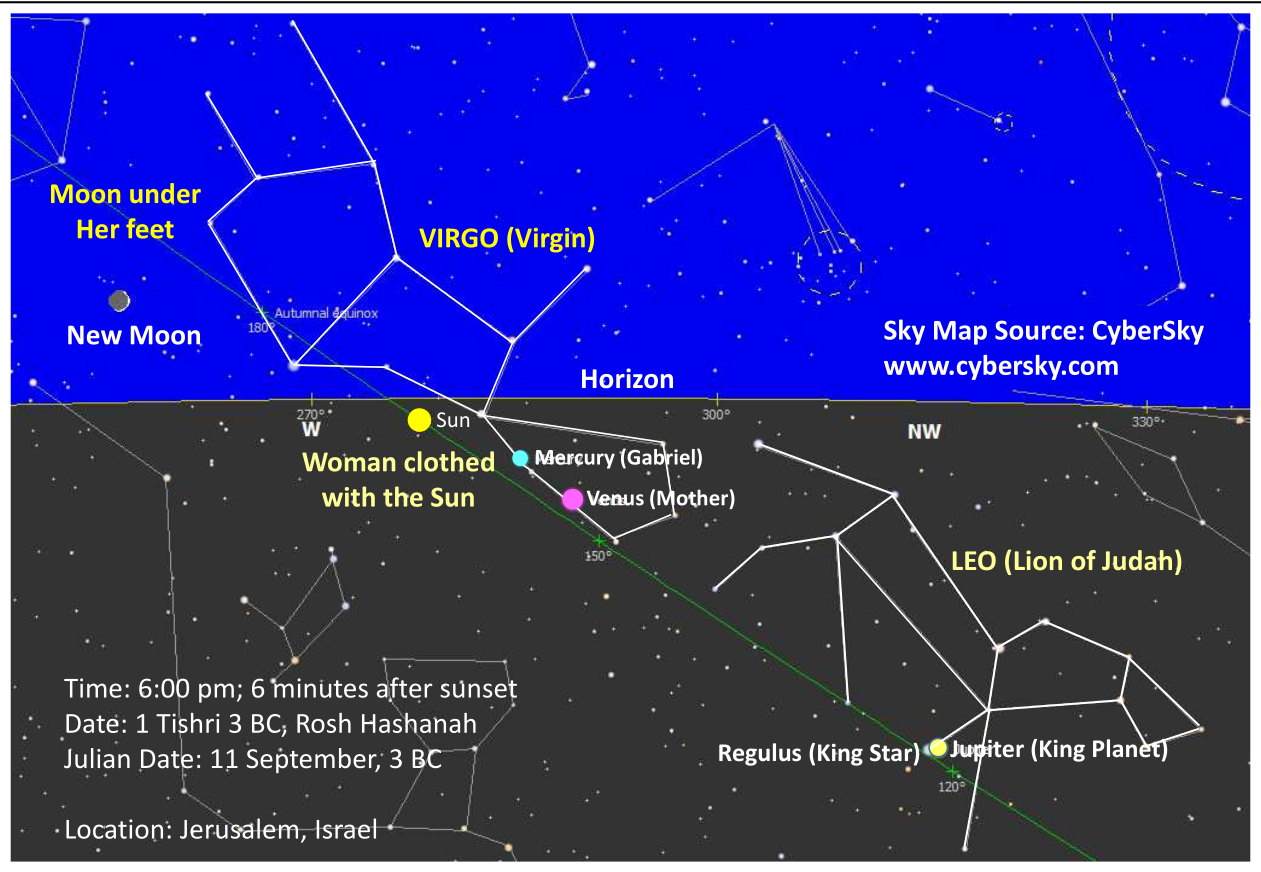
\includegraphics[width=\textwidth]{images/The-Star-of-Bethlehem}
      \end{figure}
    \end{column}

    \begin{column}{0.2\textwidth}
      \begin{figure}
        \centering
        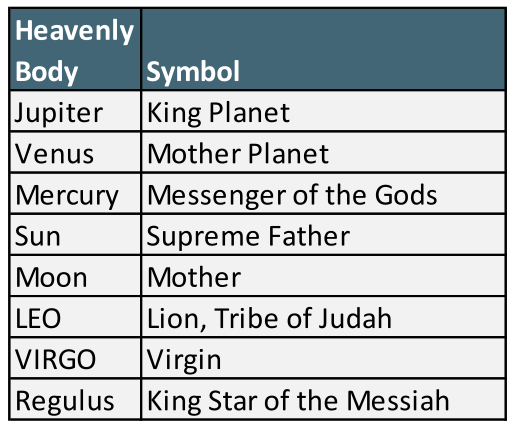
\includegraphics[width=\textwidth]{images/Heavenly-Symbolism}
      \end{figure}
    \end{column}
  \end{columns}

  天上現出大異象來:\alert{有一個婦人身披日頭,腳踏月亮,頭戴十二星的冠冕。}(\bibleref{Rv 12:1})\parvspace
\end{frame}

\begin{frame}{吹角節預表人子再臨}
  \alert{當那日,必大發角聲},在亞述地將要滅亡的,並在埃及地被趕散的,都要來,他們就在耶路撒冷聖山上敬拜耶和華。(\bibleref{Is 27:13})\parvspace
  你們要在錫安\alert{吹角},在我聖山\alert{吹出大聲}。國中的居民都要發顫;因為\alert{耶和華的日子將到,已經臨近}。(\bibleref{Jl 2:1})\parvspace
  那時,人子的兆頭要顯在天上,地上的萬族都要哀哭。\alert{他們要看見人子,有能力,有大榮耀,駕着天上的雲降臨}。他要差遣使者,用\alert{號筒的大聲},將他的選民,從四方,從天這邊到天那邊,都招聚了來。」(\bibleref{Mt 24:30-31})\parvspace
  因為\alert{主必親自從天降臨},有呼叫的聲音和天使長的聲音,又有\alert{神的號吹響};那在基督裏死了的人必先復活。(\bibleref{1Th 4:16-17})\parvspace
  第七位天使\alert{吹號},天上就有大聲音說:世上的國成了我主和主基督的國;他要作王,直到永永遠遠。(\bibleref{Rv 11:15})\parvspace
\end{frame}

\conclusion{吹角節}{人子來臨}

\topic{\texthebrew{יוֹם כִּפּוּר}}

\begin{frame}{贖罪日}
  「每逢\alert{七月初十日},你們要刻苦己心,無論是本地人,是寄居在你們中間的外人,甚麼工都不可做;這要作你們永遠的定例。\alert{因在這日要為你們贖罪,使你們潔淨。你們要在耶和華面前得以潔淨,脫盡一切的罪愆}。這日你們要守為\alert{聖安息日 (\texthebrew{שַׁבַּת שַׁבָּתוֹן})},要刻苦己心;這為永遠的定例。 那受膏、接續他父親承接聖職的祭司要穿上細麻布的聖衣,行贖罪之禮。他要在至聖所和會幕與壇行贖罪之禮,並要為眾祭司和會眾的百姓贖罪。這要作你們永遠的定例-就是因以色列人一切的罪,要一年一次為他們贖罪。」(\bibleref{Lv 16:29-34})\parvspace
  \begin{itemize}
    \item “聖安息日” 字面翻譯是 ”安息日中的安息日”,強調這是一年最神聖的一日。
  \end{itemize}
\end{frame}

\question{贖罪日發生或預言的事件}

\begin{frame}{贖罪日發生或預言的事件}
  \begin{itemize}
    \item 摩西宣告上帝已赦免以色列人拜金牛犢的罪?(\bibleref{Ex 34:29-35})\parencite{GoldenCalf, SederOlamRabbah, YomKippur}
    \item 耶穌登山變相?(\bibleref{Mt 17:1-13; Mk 9:2-13;Lk 9:28-36})\parencite{YeshuaInYomKippur}
    \item 末日審判 (\bibleref{Rv 20:11-15})
  \end{itemize}
\end{frame}

\begin{frame}{赦免以色列人拜金牛犢的罪 \textendash\ 時間線}
  \begin{itemize}
    \item 3/7: 摩西在七七節領受十戒 (\bibleref{Ex 19; 20:1-17})\parencite{TenCommandmentsOnShavuot}
    \item 3/7\textendash\ 4/17:摩西在山中\alert{四十晝夜} (\bibleref{Ex 24:18; Dt 9:11})。
    \item 4/17: 摩西下山打碎石板 (\bibleref{Ex 32:19; Dt 9:15-17})。
    \item 4/18\textendash\ 5/28: \alert{第二天},摩西上山贖罪\alert{四十晝夜} (\bibleref{Ex 32:30; Dt 9:18,25})。
    \item 5/29: \alert{清晨起來},摩西拿兩塊石板上西奈山 (\bibleref{Ex 34:4; Dt 10:3})。
    \item 6/1\textendash\ \alert{7/10}: 摩西在山上\alert{四十晝夜}重新立約 (\bibleref{Ex 34:28; Dt 10:10})。
  \end{itemize}
\end{frame}

\begin{frame}{贖罪日預表末日的審判}
  我又看見一個白色的大寶座與坐在上面的;從他面前天地都逃避,再無可見之處了。我又看見死了的人,無論大小,都站在寶座前。案卷展開了,並且另有一卷展開,就是生命冊。\alert{死了的人都憑着這些案卷所記載的,照他們所行的受審判}。於是海交出其中的死人;死亡和陰間也交出其中的死人;他們都照各人所行的受審判。\parvspace
  死亡和陰間也被扔在火湖裏;這火湖就是第二次的死。\alert{若有人名字沒記在生命冊上,他就被扔在火湖裏}。(\bibleref{Rv 20:11-15})\parvspace
\end{frame}

\conclusion{贖罪日}{末日審判}

\topic{\texthebrew{סֻכּוֹת}}

\begin{frame}{住棚節的時間}
  又要守收割節,所收的是你田間所種、勞碌得來初熟之物。並在年底收藏,要守\alert{收藏節\texthebrew{חַג הָאָסִף}} (\bibleref{Ex 23:16})\parvspace
  耶和華對摩西說: 「你曉諭以色列人說:這\alert{七月十五日是住棚節,要在耶和華面前守這節七日}。第一日當有聖會,甚麼勞碌的工都不可做。七日內要將火祭獻給耶和華。\alert{第八日當守聖會},要將火祭獻給耶和華。這是嚴肅會,甚麼勞碌的工都不可做。\parvspace
  \textellipsis{}\parvspace
  「你們收藏了地的出產,就\alert{從七月十五日起,要守耶和華的節七日。第一日為聖安息;第八日也為聖安息}。第一日要拿美好樹上的果子和棕樹上的枝子,與茂密樹的枝條並河旁的柳枝,在耶和華-你們的神面前歡樂七日。每年七月間,要向耶和華守這節七日。這為你們世世代代永遠的定例。 \alert{你們要住在棚裏七日;凡以色列家的人都要住在棚裏,好叫你們世世代代知道,我領以色列人出埃及地的時候曾使他們住在棚裏。我是耶和華-你們的神}。」(\bibleref{Lv 23:33-36})\parvspace
\end{frame}

\begin{frame}{曠野的意義}
  \begin{itemize}
    \item 曠野 (\texthebrew{מִדְבָּר})\ 的字根是話語 (\texthebrew{דָבַר}),表示曠野是領受神話語的地方。
    \item 摩西、以利亞、施洗約翰、耶穌、保羅都曾到曠野領受神的話語。
  \end{itemize}
\end{frame}

\question{住棚節發生的聖經事件}

\begin{frame}{住棚節事件}
  \begin{itemize}
    \item 所羅門獻聖殿 (\bibleref{IK 8:22-53; 2Ch 6:12-42})
    \item 被擄歸回慶祝住棚節 (\bibleref{Ne 8:13-18})
    \item 耶穌活水的江河 (\bibleref{Jn 7:37-39})\parencite{YeshuaInSukkot}
    \item 神與我們同在 (\bibleref{Rv 21:1-4})
  \end{itemize}
\end{frame}

\conclusion{住棚節}{\texthebrew{עִמָּנוּאֵל}}

\begin{frame}[allowframebreaks]
  \frametitle{參考文獻}
  \printbibliography
\end{frame}

\end{document}
